\section{Results and Discussion}
\label{ch3:sec:results}

\subsection{Time-series evolution}
\label{ch3:subsec:time-series-evolution}

The objective of the smart-charging algorithm is to distribute the charging demand of a fleet of EVs over the underlying base demand in such a way that no additional demand spikes are produced.
After assigning each EV's energy demand to its initially known demand trough, the algorithm produces a new demand spike since all EVs are charging simultaneously.
Through repetitive iterations and reallocating a portion of the assigned energy to different demand troughs, the algorithm is then able to spread all EVs' demands to form a flat demand profile in the end.
This process is shown in Figure \ref{ch3:fig:time-series}.

\begin{figure}\centering
	\subfloat[]{
		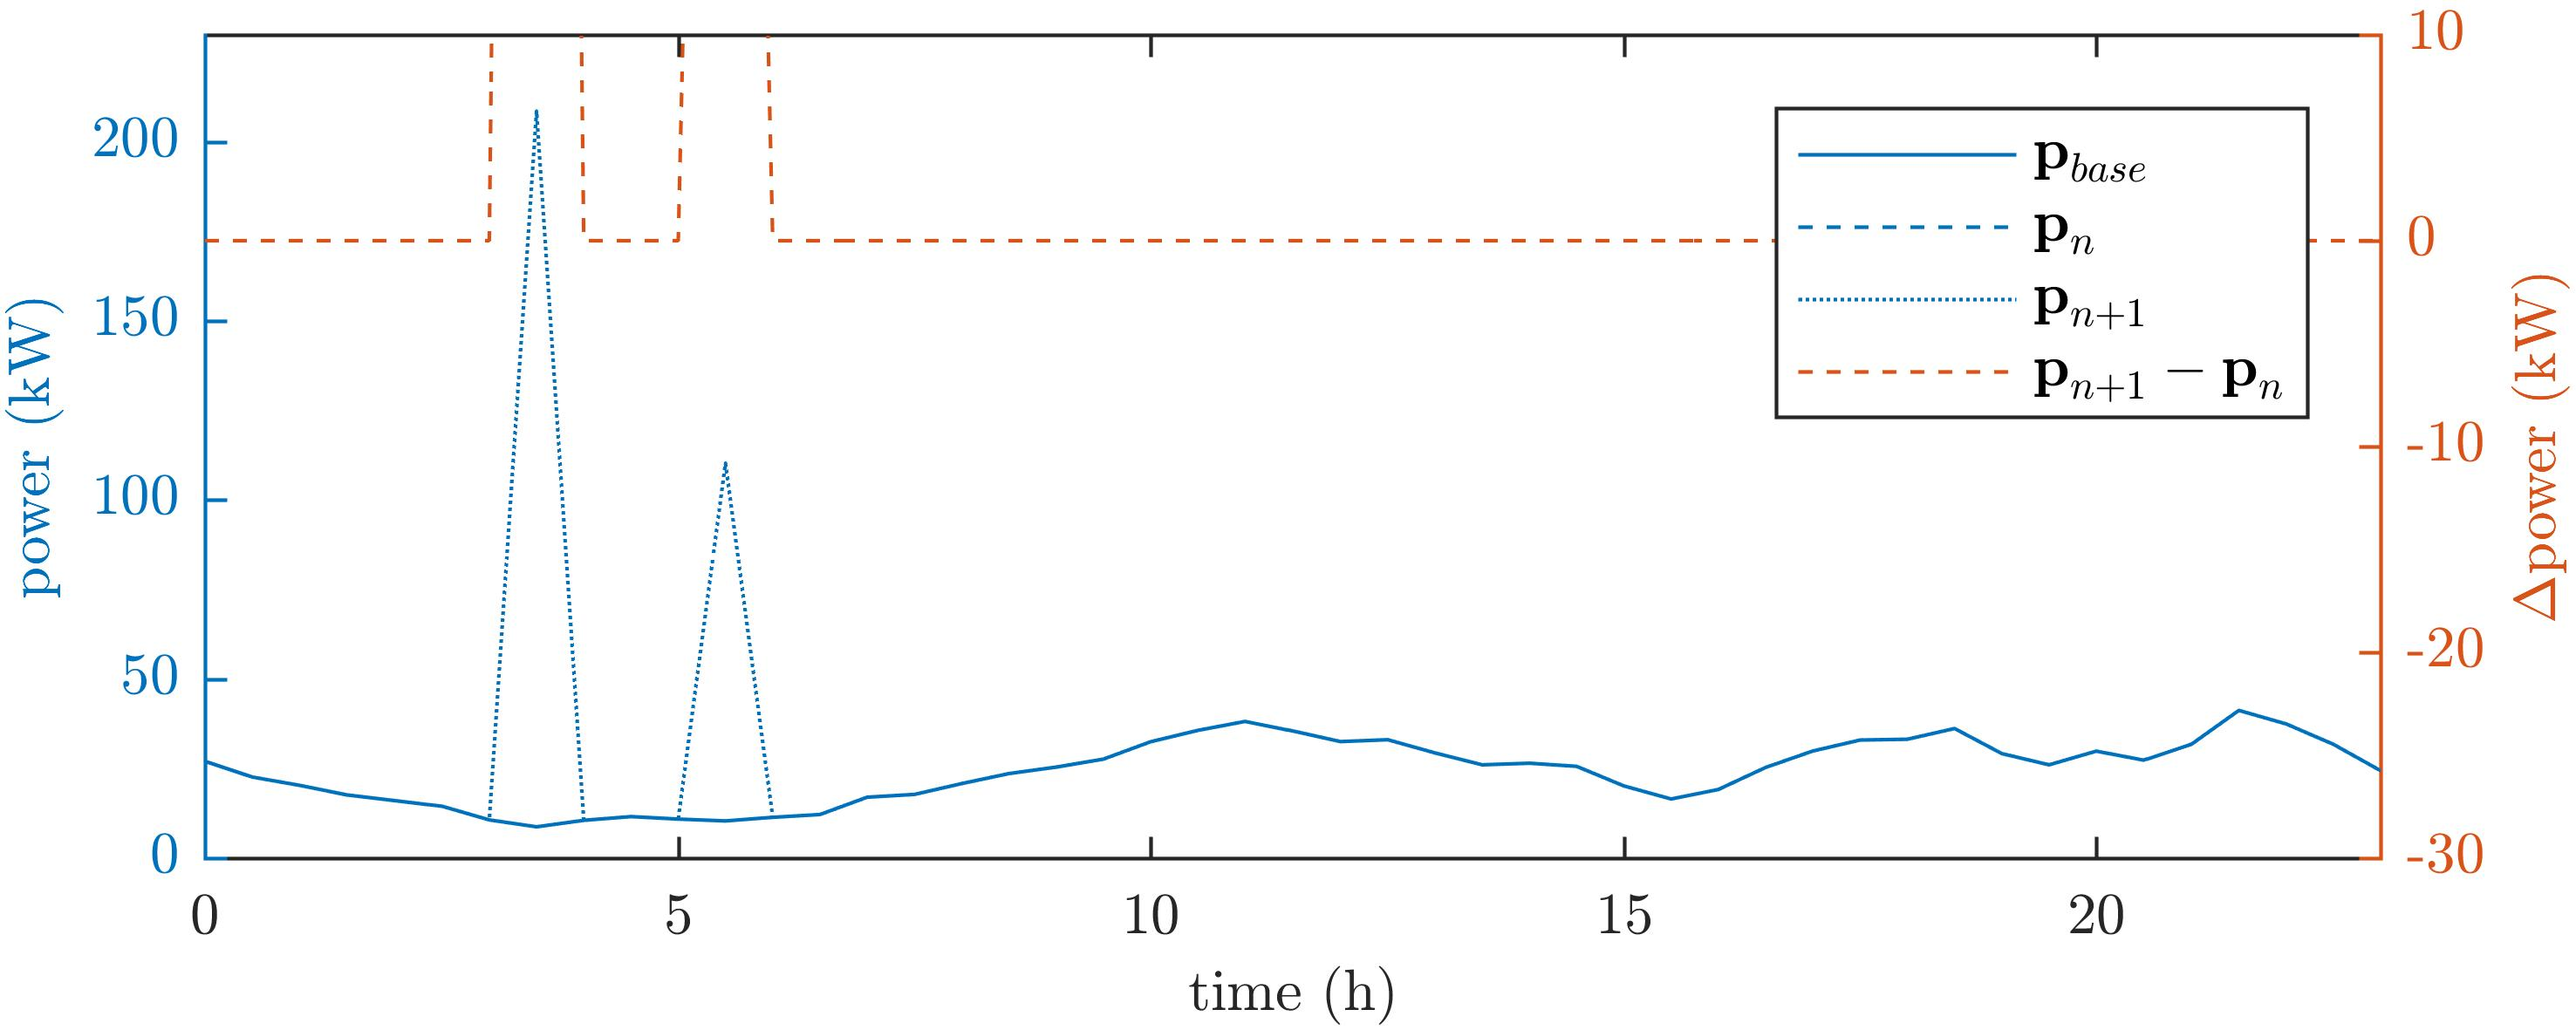
\includegraphics[height=4.5cm]{_chapter3/fig/time-series/ts-i0001}
		\label{ch3:subfig:time-series-1}
	}\\
	\subfloat[]{
		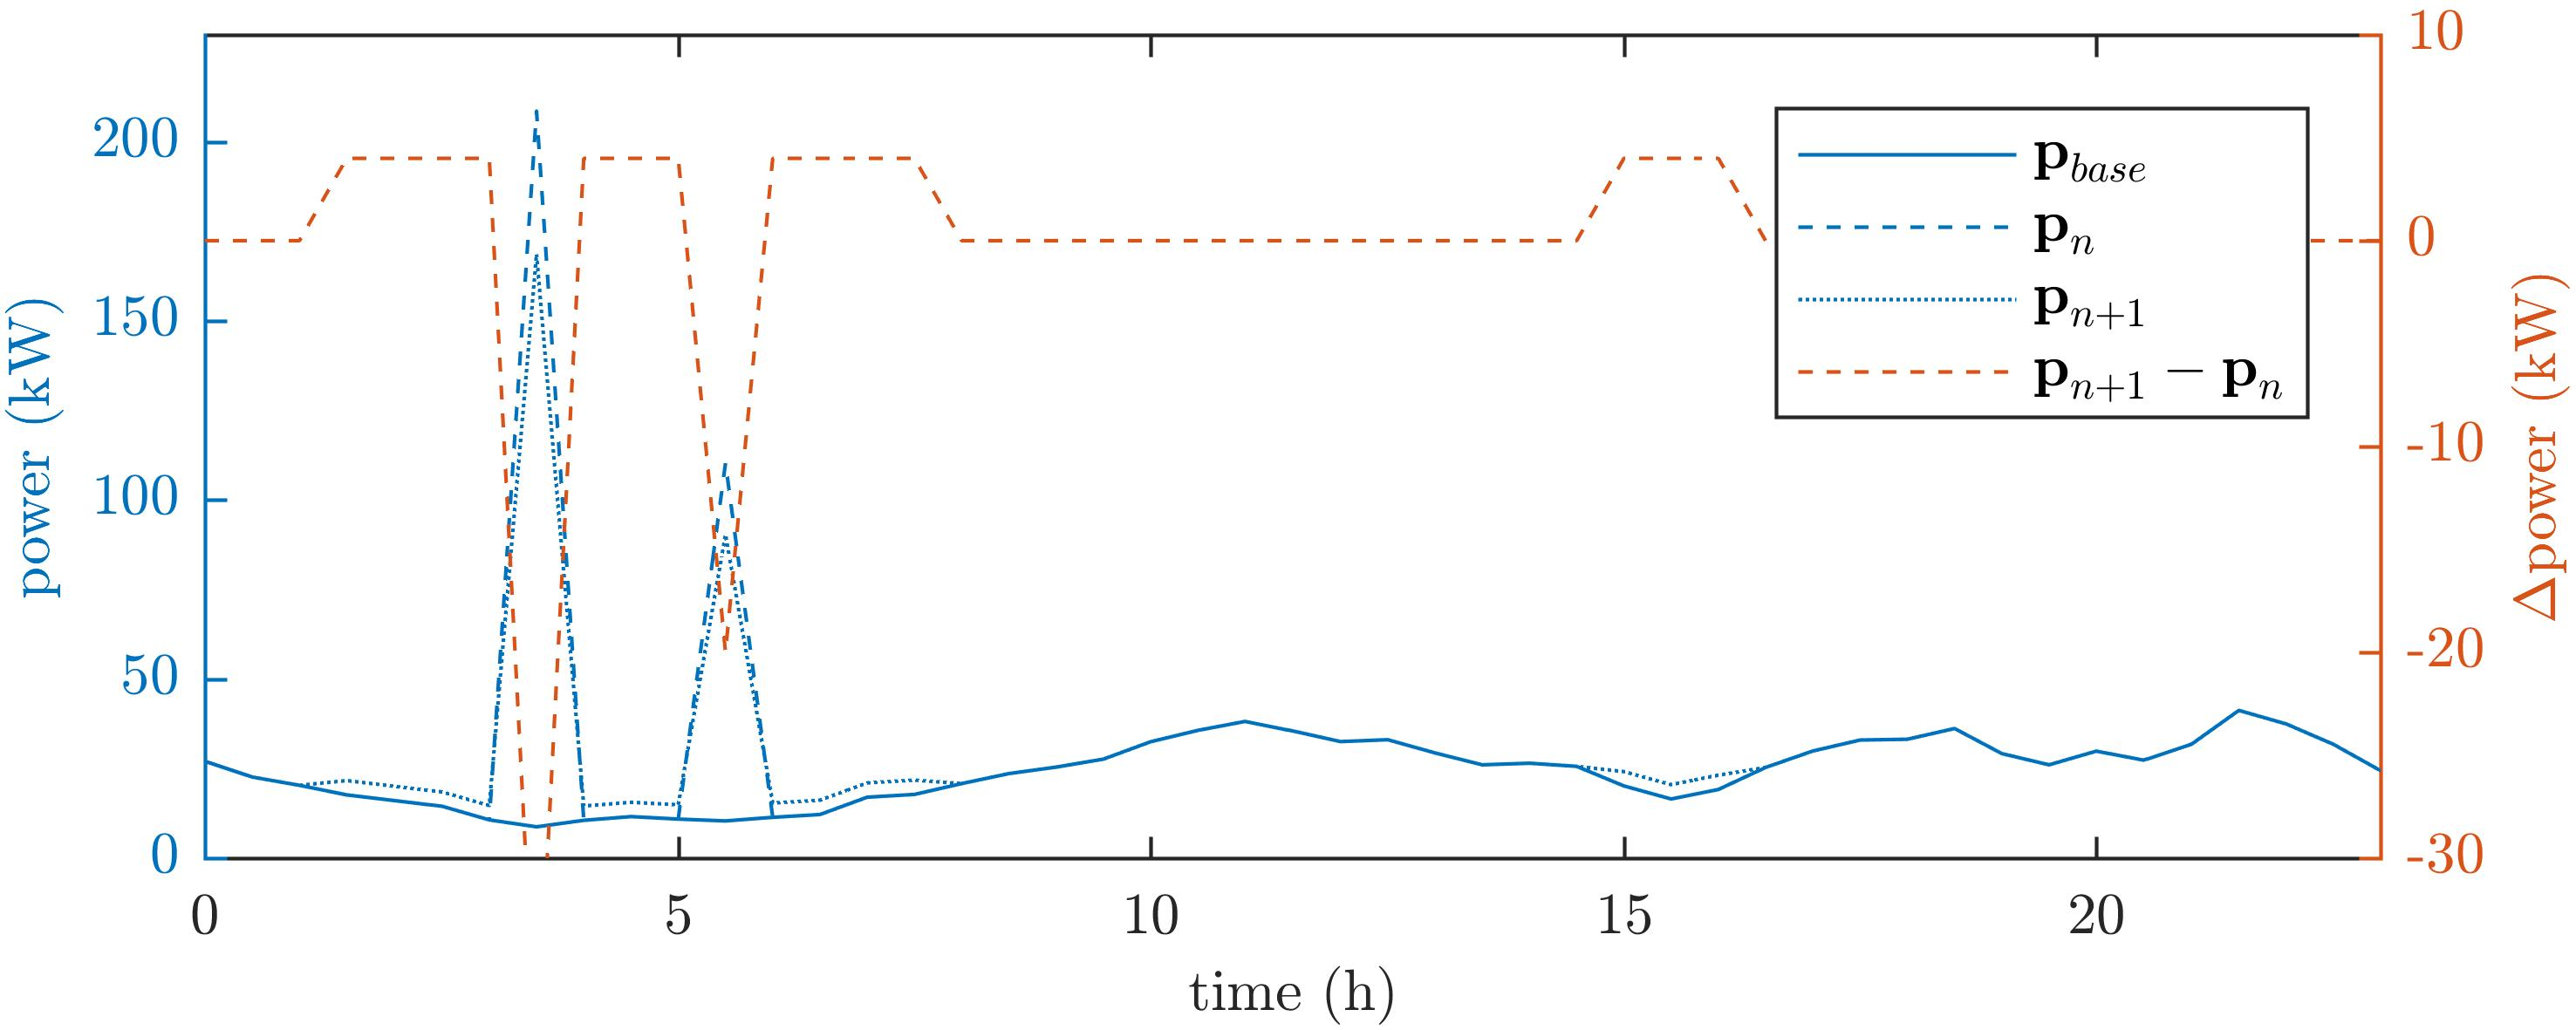
\includegraphics[height=4.5cm]{_chapter3/fig/time-series/ts-i0002}
		\label{ch3:subfig:time-series-2}
	}\\
	\subfloat[]{
		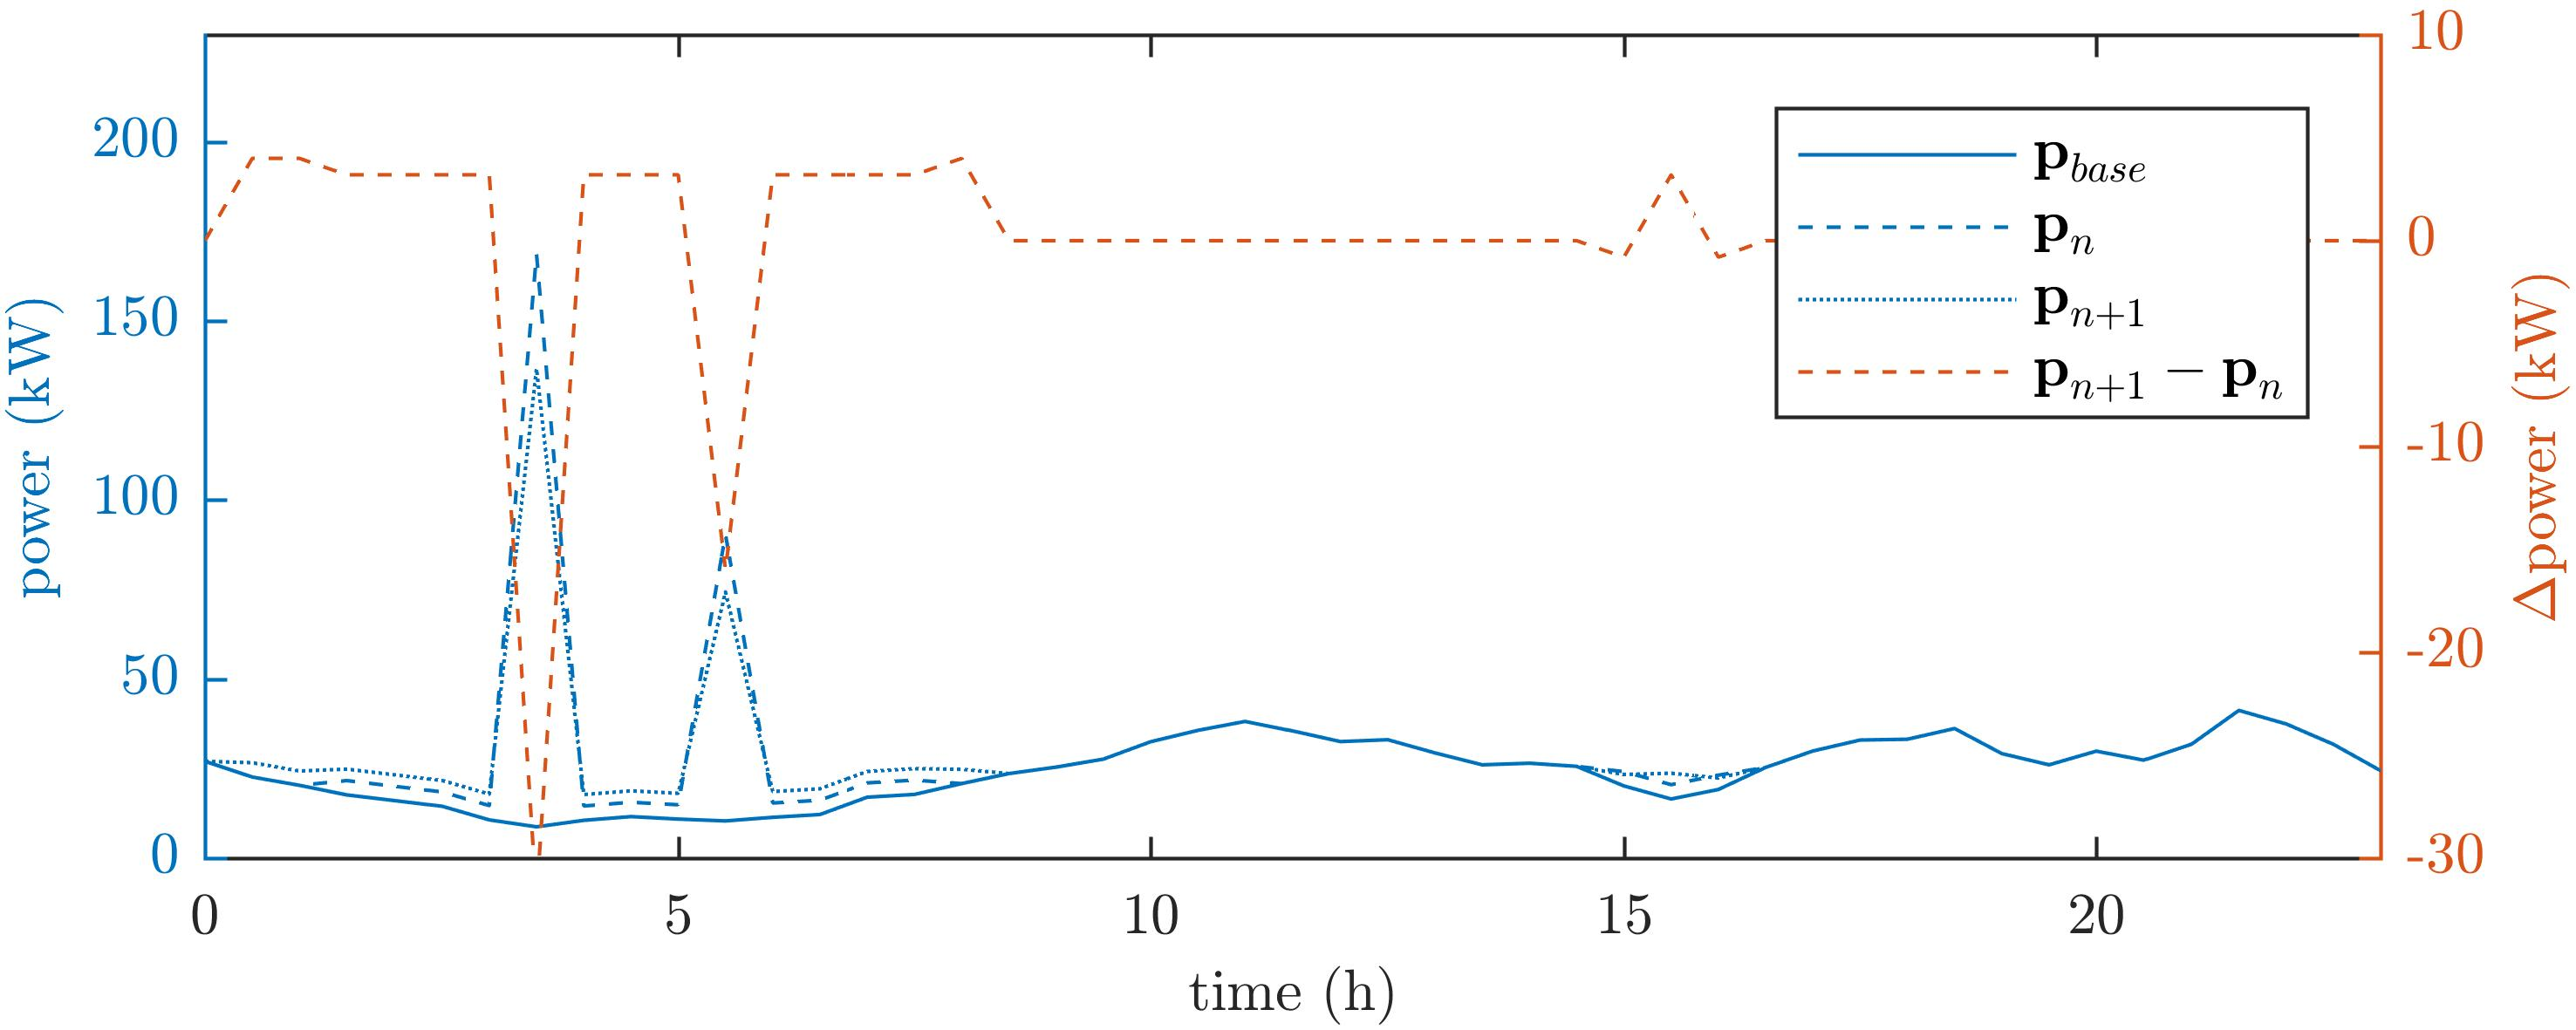
\includegraphics[height=4.5cm]{_chapter3/fig/time-series/ts-i0003}
		\label{ch3:subfig:time-series-3}
	}\\
	\subfloat[]{
		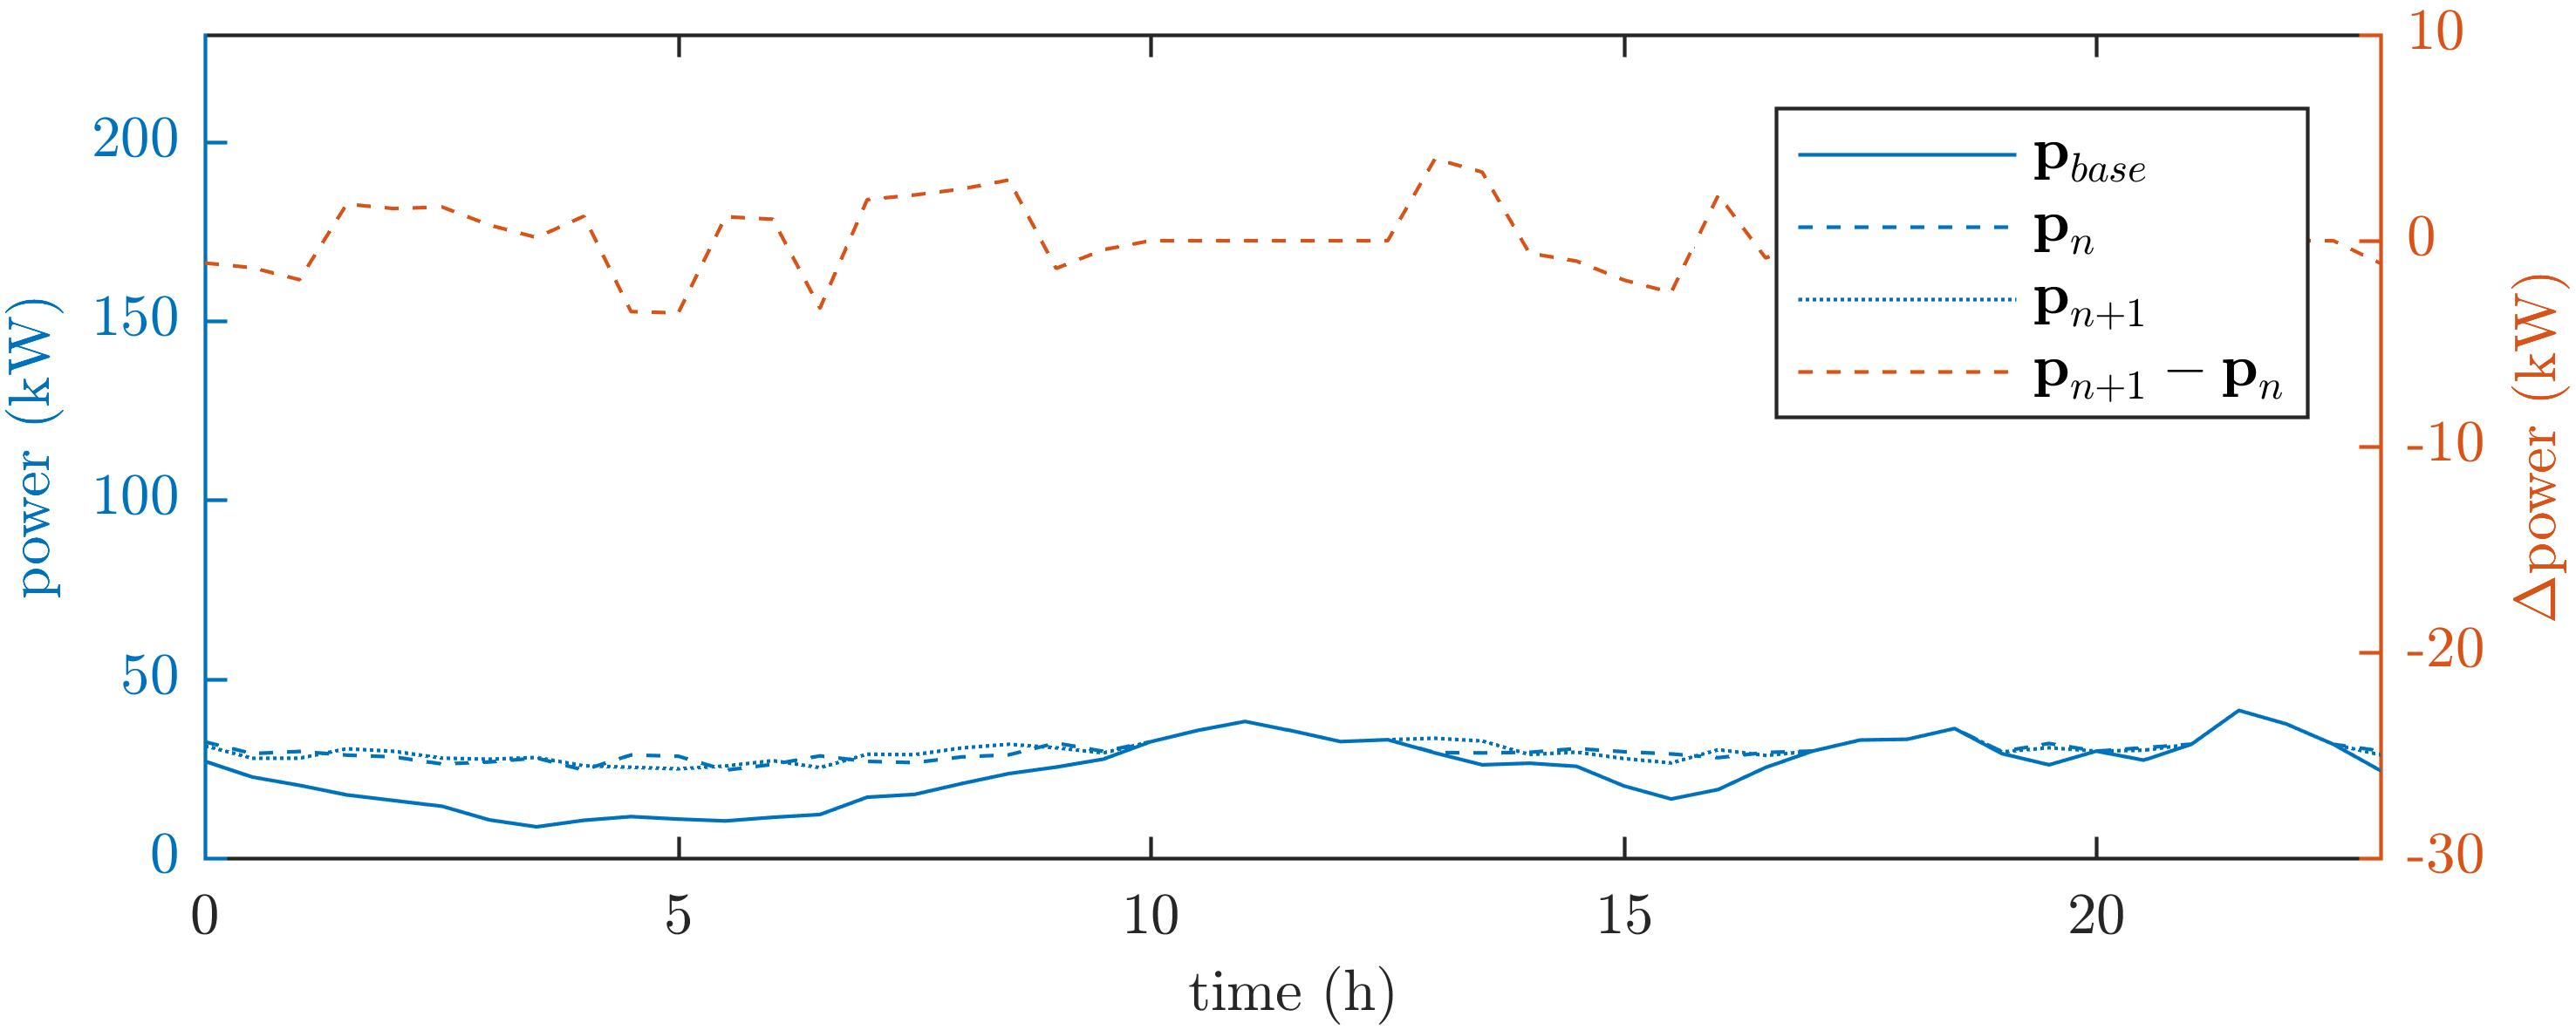
\includegraphics[height=4.5cm]{_chapter3/fig/time-series/ts-i0100}
		\label{ch3:subfig:time-series-last}
	}
\caption{Time series evolution for $\alpha=0.02$ and $\beta=0.20$, where (a) is at $n=1$, (b) is at $n=2$, (c) is at $n=3$, and (d) is at $n=N-1$.}
\label{ch3:fig:time-series}
\end{figure}

Here, the first algorithm iteration is shown in Figure \ref{ch3:subfig:time-series-1}, where allocated power profile produces two new morning spikes of around 200kW and subsequently 110kW.
The second iteration however reduces these spikes by the factor $\alpha$ (i.e $0.2$) and redistributes the undone charging powers over the new power profile.
Figure \ref{ch3:subfig:time-series-2} shows this reduction and reallocation.
Figure \ref{ch3:subfig:time-series-3} is the third iteration that reduces and redistributes the peaks even further.
In the end, i.e. when $n=N$, the resulting power profile becomes as flat as possible, which is shown in Figure \ref{ch3:subfig:time-series-last}.
Throughout these iterations, it can be observed how the peak load in the total power, i.e. $\textbf{p}_n$, reduces and it can be observed how the changes in charging power, i.e. $\textbf{p}_{n+1}-\textbf{p}_n$, reduce in variance, which indicates that the algorithm works for the chosen parameters of $\alpha$ and $\beta$.
However, different parameters of $\alpha$ and $\beta$ do impact the performance of this synchronised algorithm execution, as shown in Figure \ref{ch3:fig:oscillation}.

\begin{figure}\centering
	\subfloat[]{
		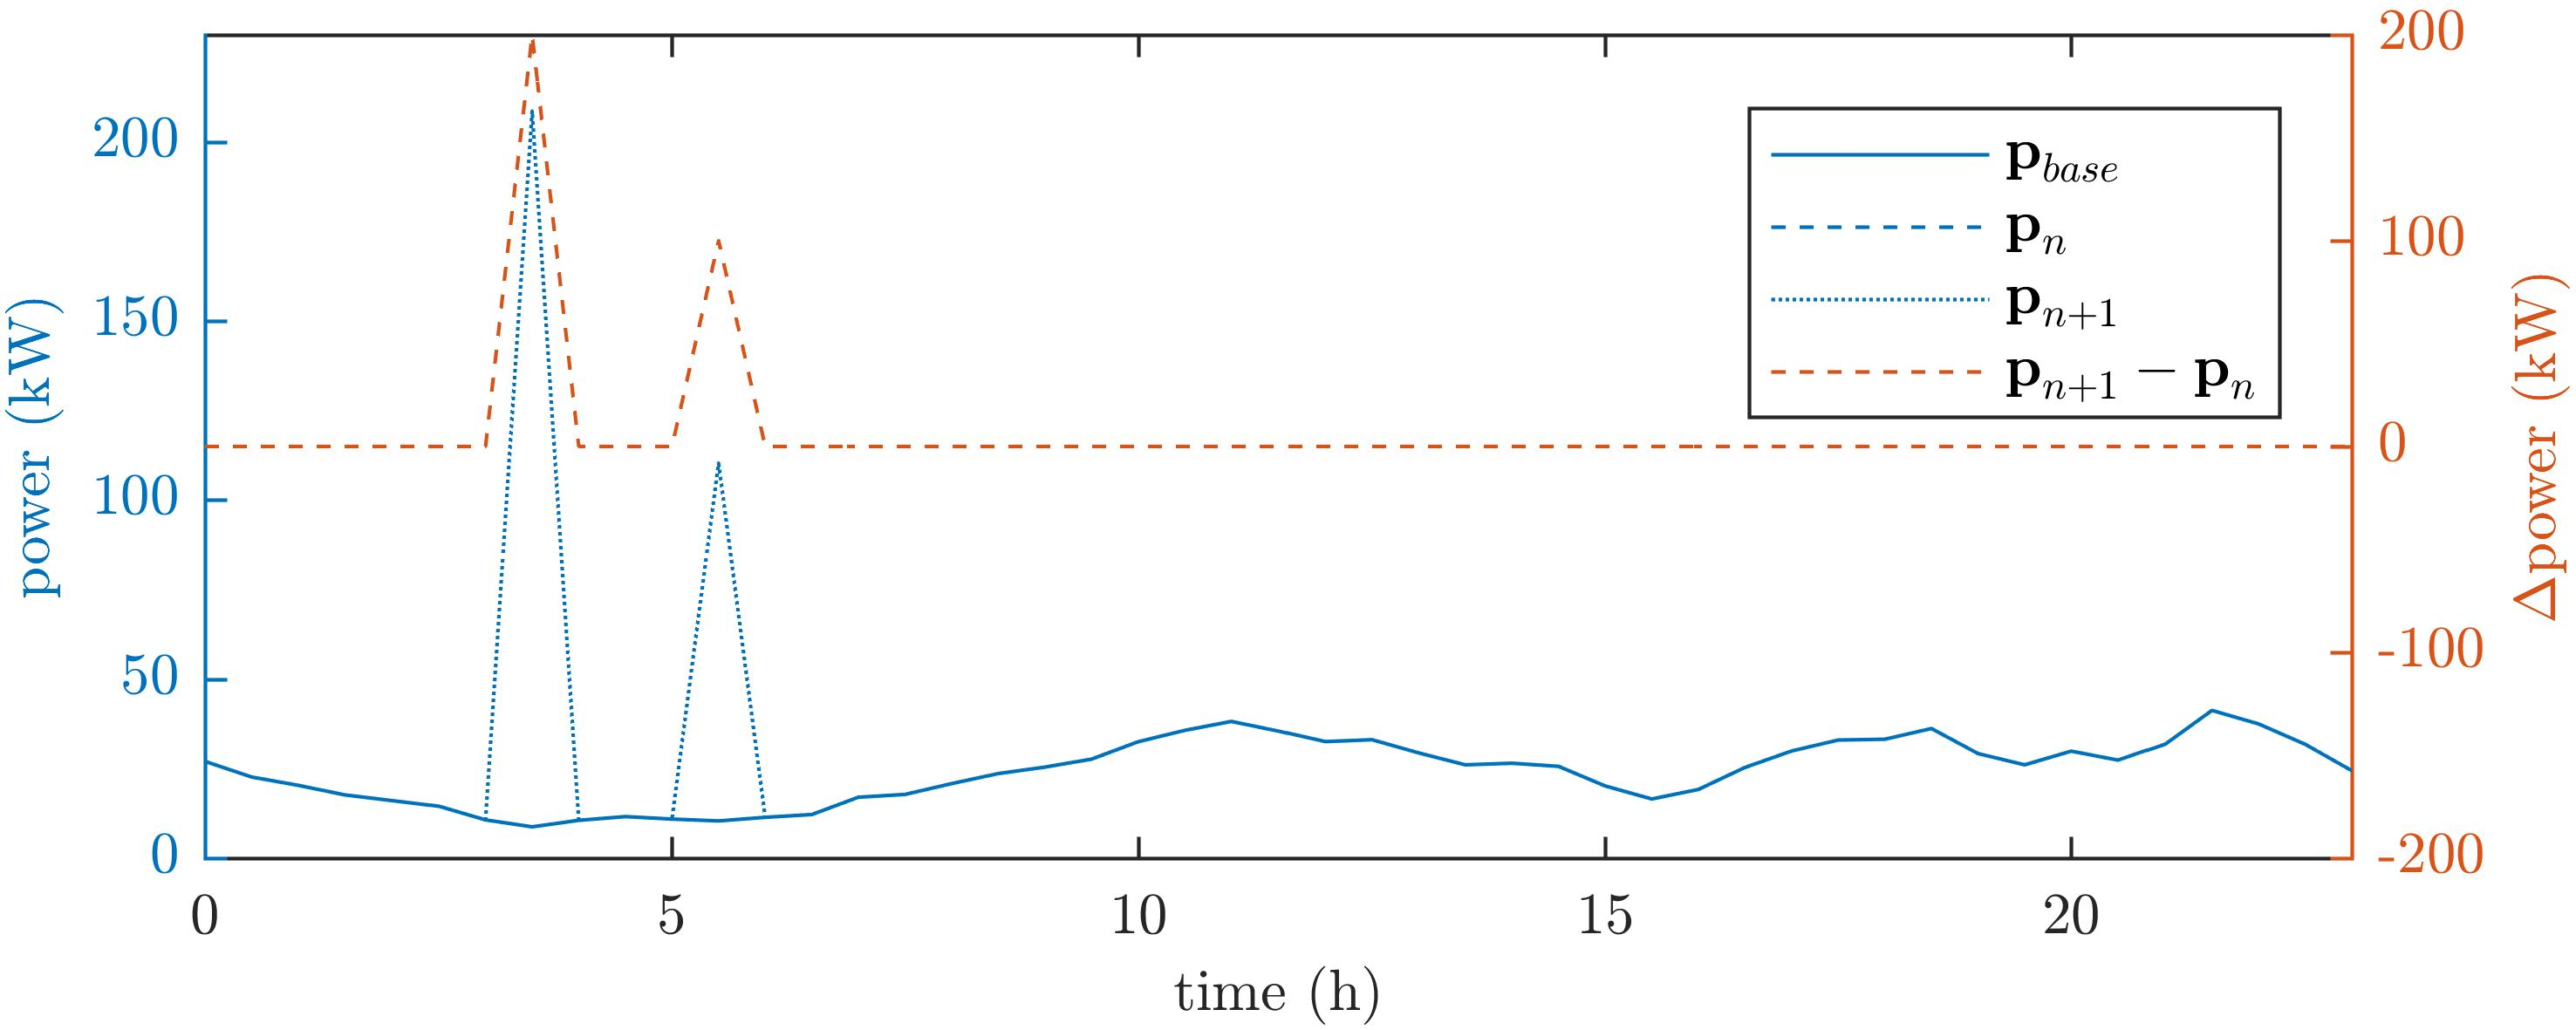
\includegraphics[height=4.5cm]{_chapter3/fig/oscillation/ts-i0001}
		\label{ch3:subfig:oscillation-1}
	}\\
	\subfloat[]{
		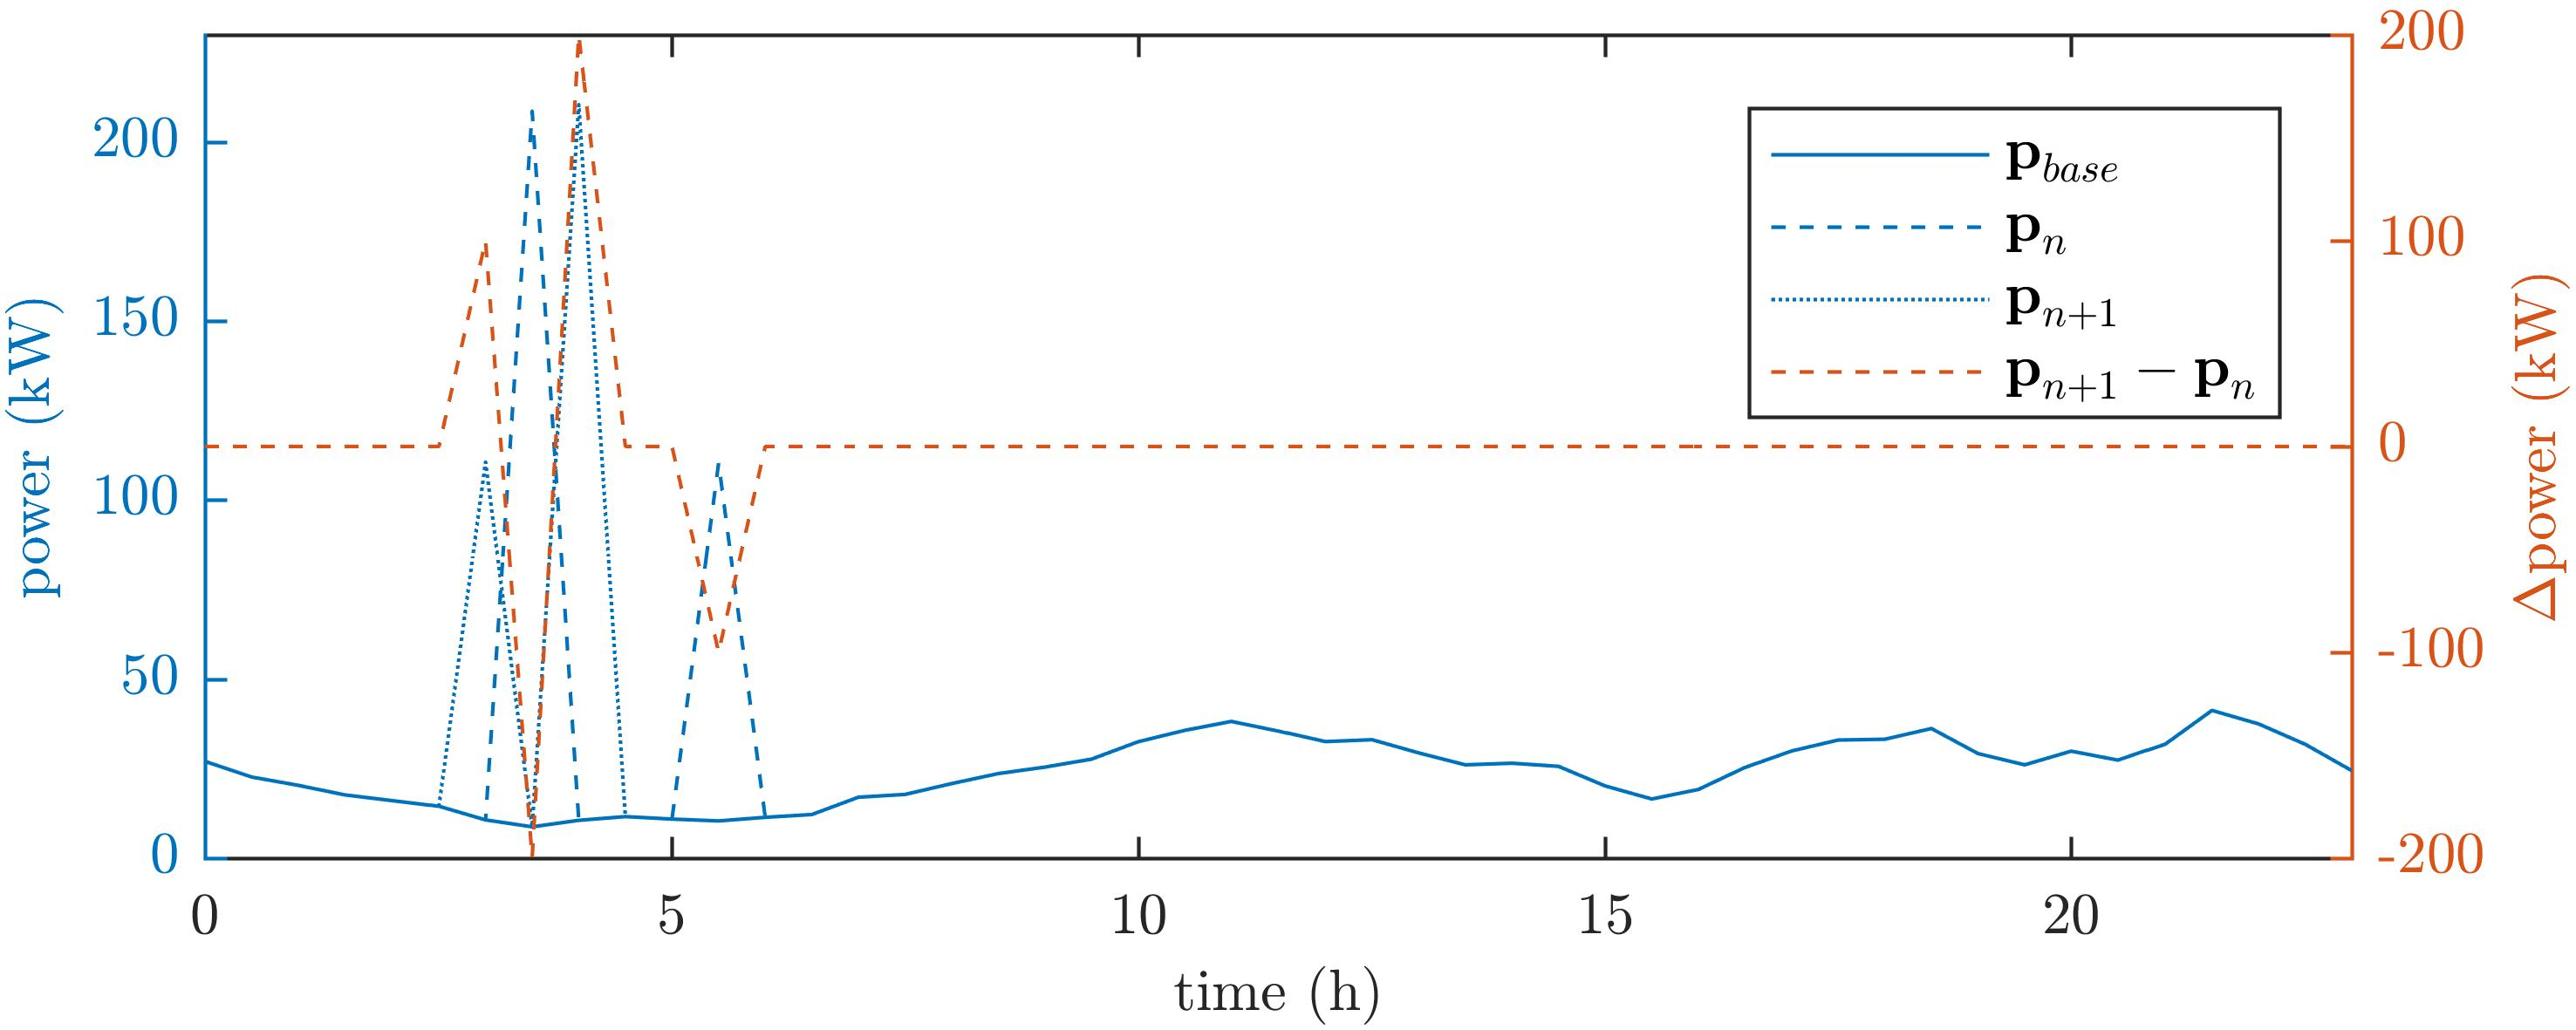
\includegraphics[height=4.5cm]{_chapter3/fig/oscillation/ts-i0002}
		\label{ch3:subfig:oscillation-2}
	}\\
	\subfloat[]{
		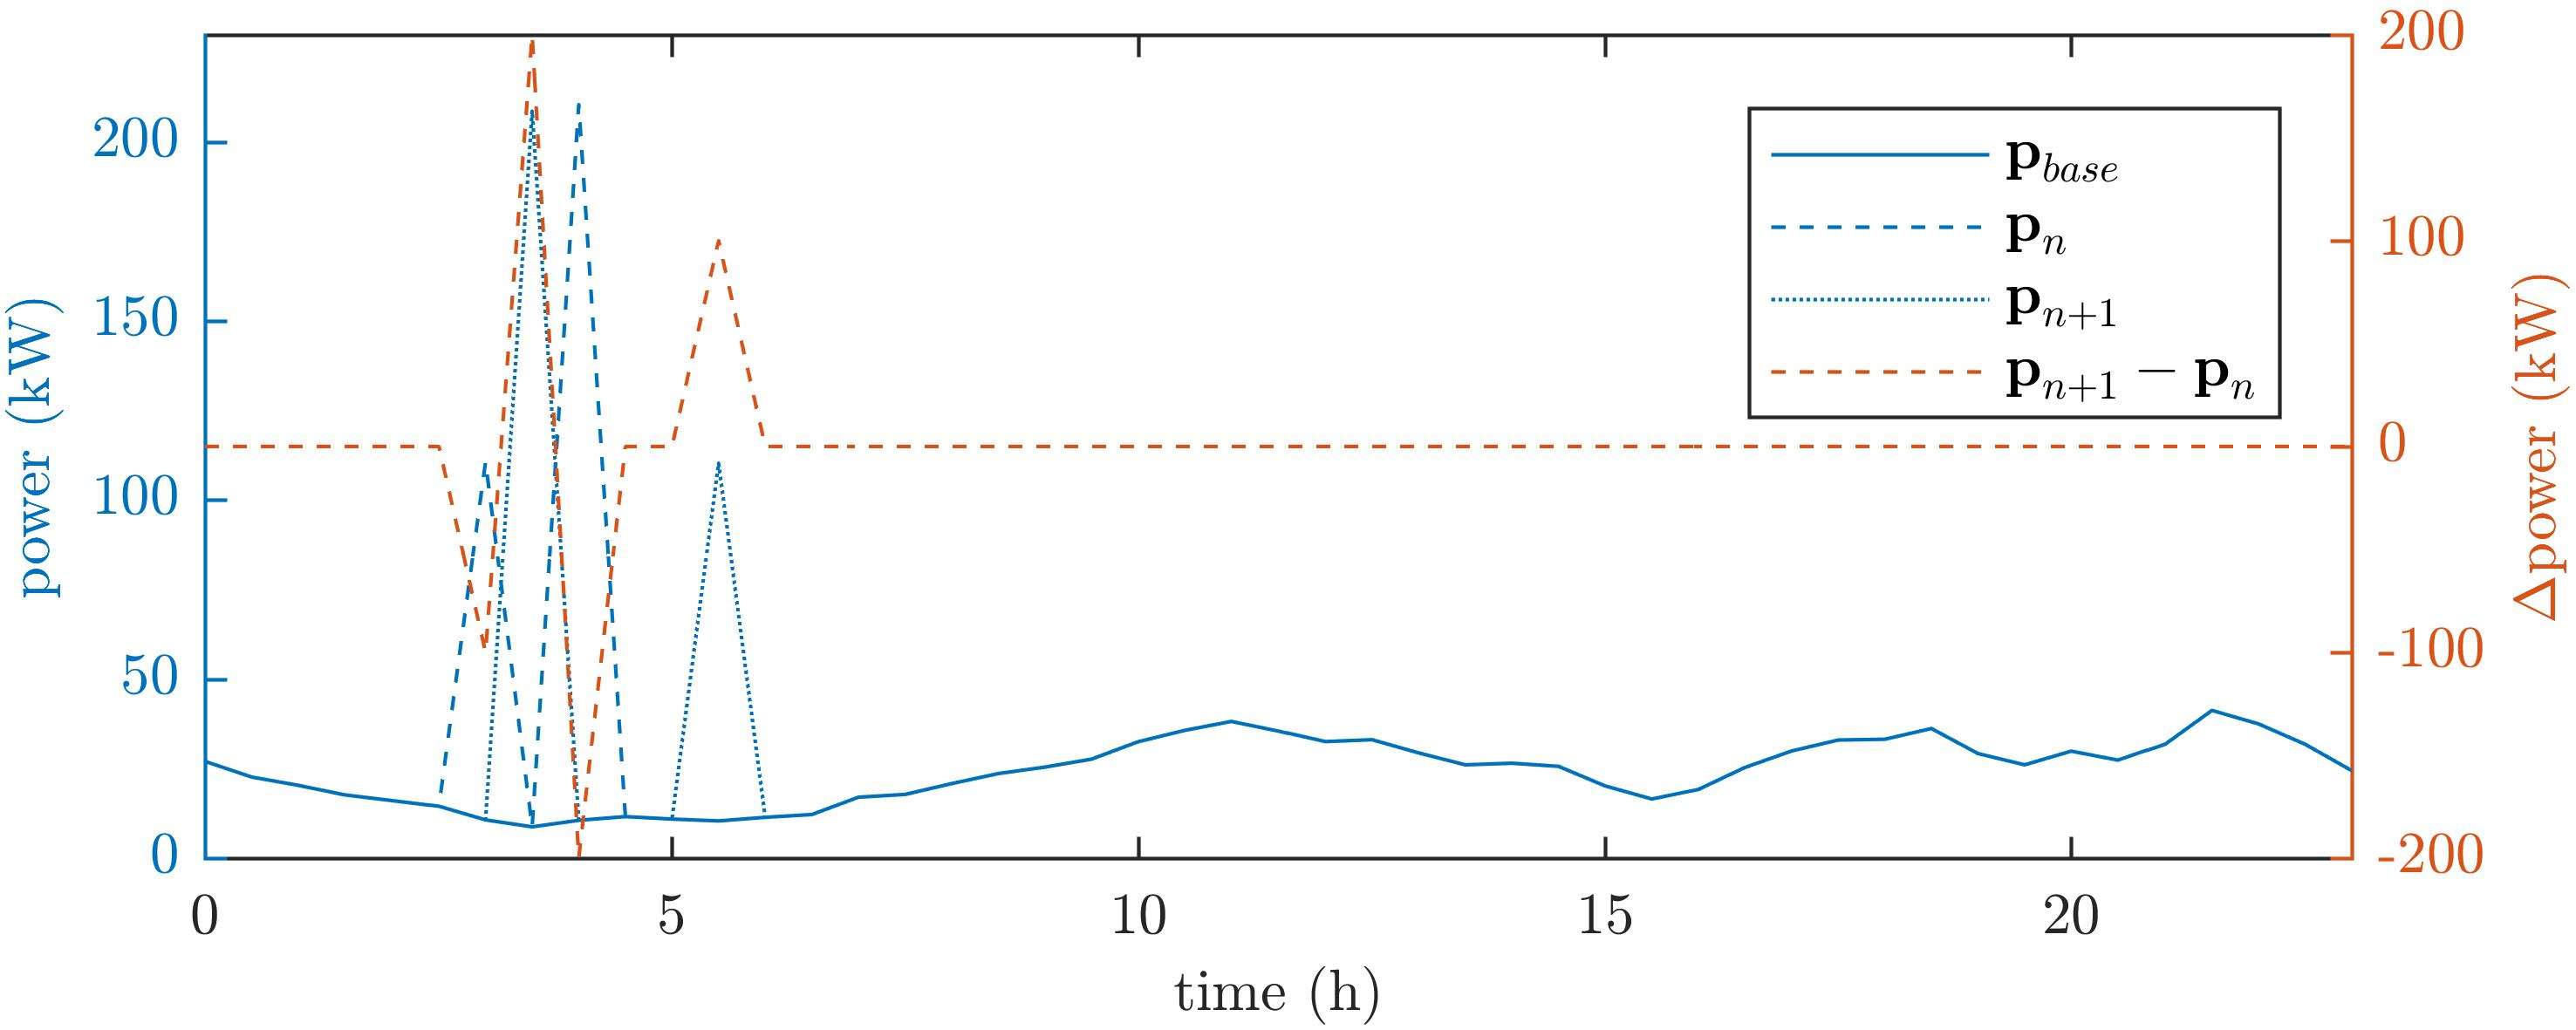
\includegraphics[height=4.5cm]{_chapter3/fig/oscillation/ts-i0003}
		\label{ch3:subfig:oscillation-3}
	}\\
	\subfloat[]{
		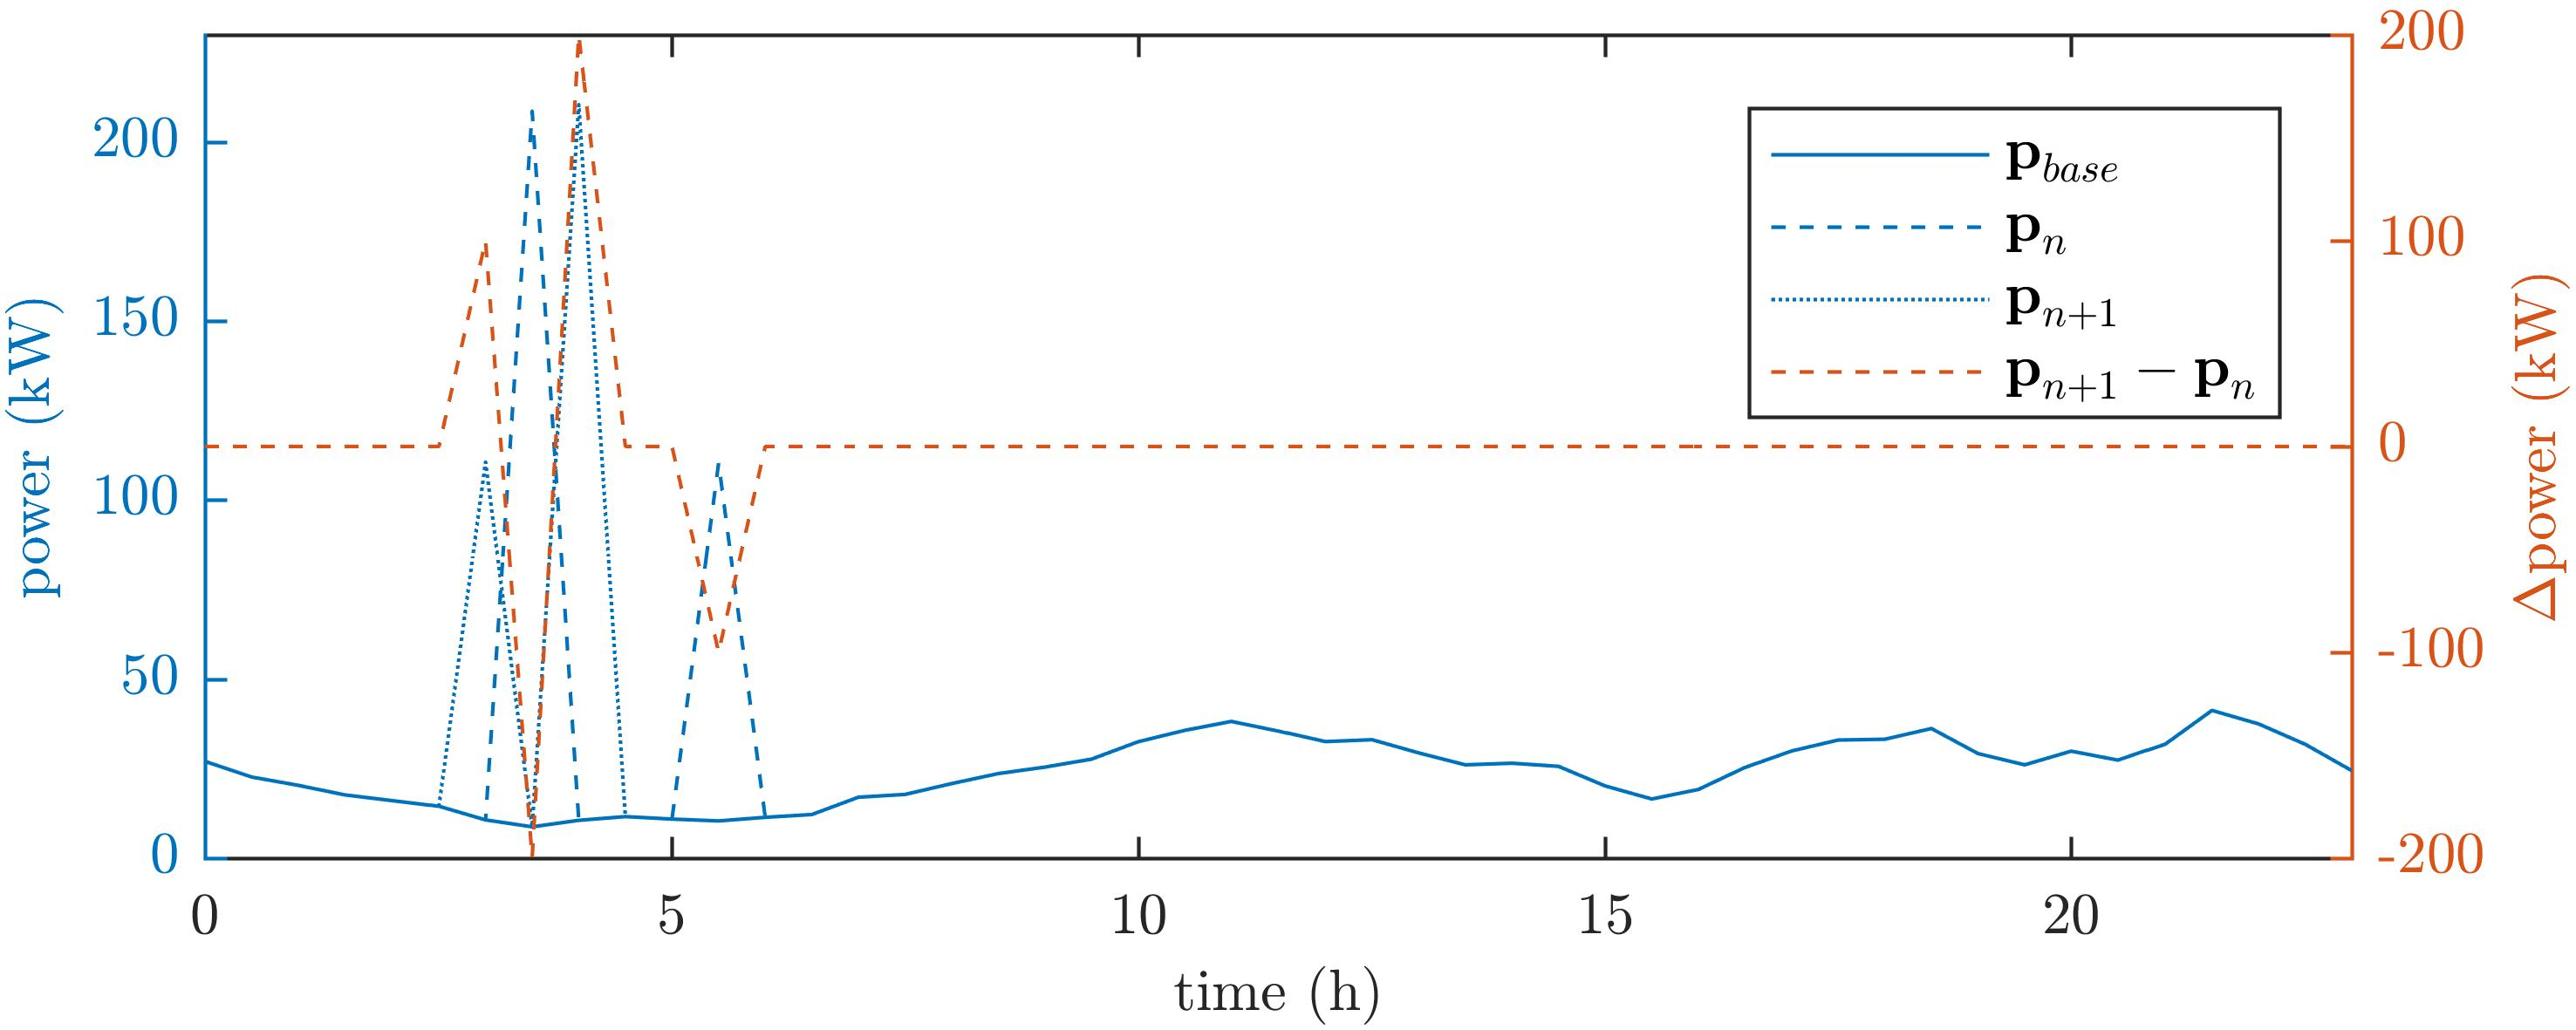
\includegraphics[height=4.5cm]{_chapter3/fig/oscillation/ts-i0100}
		\label{ch3:subfig:oscillation-last}
	}
\caption{Time series evolution for $\alpha=1.00$ and $\beta=1.00$, where (a) is at $n=1$, (b) is at $n=2$, (c) is at $n=3$, and (d) is at $n=N-1$.}
\label{ch3:fig:oscillation}
\end{figure}

